\documentclass[11pt]{article}
\usepackage[utf8]{inputenc}
\usepackage[spanish]{babel}
\usepackage{dirtytalk}
\usepackage{url}
\usepackage{amsfonts}
\usepackage{amsmath}
\usepackage{graphicx}
\usepackage{url}
\usepackage[numbers]{natbib}
\bibliographystyle{plainnat}
\usepackage{booktabs}
\usepackage[toc,page]{appendix}
\usepackage{bm}

\usepackage{caption} % To make fonts on figure smaller
\captionsetup[figure]{font=small}
\captionsetup[table]{font=small}


\title{Introducción al Machine Learning \\ \large \texttt{S01: Nociones Básicas}}
\author{Edmundo Avendaño Mejía\\Gerardo Durán Martín}
\begin{document}
\maketitle

\newcommand{\Rnums}{\mathbb{R}}

En este curso se introducirá las matemáticas detrás de machine learning. Se asume que al alumno tiene nociones de cálculo multivariado, álgebra lineal y probabilidad. Sin embargo, se repasarán conceptos importantes para poder entender el curso. Machine Learning es una rama muy extensa de estudio, por lo que se buscará introducir los algoritmos y las ideas esenciales que servirán para entender estudios recientes 

\section{¿Qué es \textit{Machine Learning}?}

Piensa en la última vez que le pediste algo a Siri, cuando tuviste que entender algo en Google Translate o Amazon te recomendó tu siguiente compra. Estos son algunos ejemplos del poder que tienen los algoritmos de aprendizaje de máquina. En este curso introduciremos las matemáticas que hacen poderosos estos algoritmos de computación incluso, algunos, más inteligentes que un humano.\\

Parafraseando a \cite{samuel}, \say{[\textbf{machine learning}], es la rama de estudio que le da a las computadoras la habilidad de \textit{aprender} sin la necesidad de ser explícitamente programadas.}. Pero, ¿con qué nos referimos a aprender? y ¿por qué no programar directamente los problemas?\\

Enfoquémonos primero en la programación de problemas. Resulta ser que existen problemas fáciles para un humano desarrollar, más no para una máquina. Pensemos en el problema de reconocer la cara de uno de tus amigos; escuchar la voz de tus padres y saber que son ellos; o incluso poder hacer el resumen de alguna lectura. Todos estos son problemas que son fáciles para los humanos, sin embargo, tratar de programar bajo \textit{métodos tradicionales} alguno de estos problemas se vuelve una tarea ardua o incluso imposible. Tareas triviales para para nosotros no lo son para un computadora necesariamente. En ese caso, ¿cómo le podríamos enseñar a una computadora las habilidades que poseemos?\\

Esto último nos lleva de nuevo a la pregunta ¿cómo le enseñamos a una computadora? De una manera formal, \say{un programa de computación se dice aprende de una experiencia \textbf{E}, respecto a una clase de tarea \textbf{T} y medida de desempeño \textbf{P}, si el desempeño en \textbf{T}, medido bajo \textbf{P} mejora con \textbf{E}}\cite{Mitchell}. \\


La definición planteada podría parecer un poco rebuscada, sin embargo, considera tres factores necesarios para definir aprendizaje de una manera concreta y cuantitativa.

\section{La tarea \textbf{T}}
El aprendizaje sin alguna meta sobre la cuál aplica el conocimiento es inservible. Para nosotros humanos, aprender a cantar, a programar o recordar las instrucciones para algún platillo tienen un fin (\textbf{T}): dejar de cantar mal, crear una aplicación o cocinarle a alguien. En el contexto de machine learning sucede lo mismo, si tuviéramos un robot, $T$ podría ser que aprenda a tocar la guitarra; si trabajamos en Facebook, $T$ sería poder reconocer a cada una de las personas en una foto y decir quienes son, dar recomendaciones de posibles amigos o incluso, recomendarte una noticia o lectura que sea de tu agrado; para un banco, $T$ podría ser reconocer transacciones fraudulentas de tarjetas de crédito; etc.\\

Lo primero antes de aplicar la inteligencia artificial es tener una meta (o problema) sobre el cuál deseemos trabajar. Así como no aprenderías a cocinar para ser el mejor resolviendo integrales, no querrías aplicar un problema de regresión para clasificar. Consideremos algunas tareas más generales propuestas por \cite{Goodfellow-et-al-2016} :
\begin{itemize}
	\item Clasificación ($f: \Rnums^n \to C$; $C = \{c_1, \ldots, c_k\}$). La tarea de clasificar la podemos considerar como una función cuyo \textit{input} es un vector de valores y el \textit{output} un elemento de una clase discreta. En ese sentido, reconocer una cara sería un problema de clasificación, el \textit{input} de nuestra función sería la imagen de una personas mientras que el \textit{output} sería el nombre de la persona en la imagen.
	\item Regresión ($f: \Rnums^n \to \Rnums^m$). A diferencia de la clasificación, el \textit{output} en un problema de regresión sería un vector de $m$ entradas en los números reales.
	\item \textit{Machine Translation} se encarga de traducir de un idioma a otro. El \textit{input} de nuestra función sería un texto o una voz y el \textit{output} el idioma del que se trate, la traducción o alguna tarea relacionada.
	\item \textit{Detección de anomalías} se encarga de poder encontrar, dentro de un sistema, elementos atípicos a lo que se consideraría normal.
	\item \textit{Dimensionality Reduction} se encarga, como su nombre dice, de reducir las dimensiones de un vector entrada. Podríamos definir esta clase de problemas como una función $f: \Rnums^m \to \Rnums^n$; $m > n$. 
\end{itemize}

\section{La experiencia \textbf{E}}
En machine learning, la experiencia \textbf{E} está dada por los datos sobre los cuales entrenaremos el modelo. En la era del \textit{big data}, mientras más datos tengamos (limpios  y relevantes al problema), mejor nuestro modelo se desempeñará\footnote{Salvo por unos detalles que veremos más adelante}. El tipo experiencia requerida depende del tipo de problema que deseemos solucionar. En general, estos problemas se dicen ser del tipo \textbf{Supervised Learning} o \textbf{Unsupervised Learning}.\\

No existe un consenso exacto entre un tipo de problema y otro. Para algunos problemas, la línea entre \textit{supervised} o \textit{unsupervised} learning puede ser muy pequeña. Sin embargo, para propósitos de este curso, consideraremos los problemas de \textit{supervised learning} como aquellos cuya base de datos sobre la cuál entrenaremos el modelo contiene características (o \textit{features}) y un objetivo asociado. El problema de saber la probabilidad de impago de una persona hacía un préstamo es un ejemplo de supervised learning, las características, serían la edad de la persona, si estudia, su género, si trabaja, etc. Por otro lado, el objetivo asociado sería conocer la probabilidad de impago. Para este tipo de problemas tratamos de encontrar, implícitamente, $\mathbb{P}(y|X)$.\\

Los problemas de \textit{unsupervised learning} serán aquellos de los cuales solo conocemos sus características, mas no un objetivo asociado, lo cual involucra conocer la topología o estructura de los datos observados. Segregar, de alguna manera, compradores dependiendo de sus gustos caería dentro de esta familia de problemas. Para este tipo de problemas tratamos de entender $\mathbb{P}(X)$.



\section{El desempeño \textbf{P}}
Creer poder hacer una tarea no implica realizarla correctamente. Al estudiar para una materia, nuestro desempeño se ve reflejado, de alguna manera, en la calificación que tengamos en el examen, más dentro de esta influyen varios factores como lo son el estado de ánimo, cuánto dormimos, etc. En general evaluar el desempeño en la vida real no es tarea fácil, lo mismo sucede en machine learning. En varias ocasiones, la métrica de desempeño \textbf{P} (o \textbf{función objetivo}) es tan importante como la tarea a realizar.\\

Como un primer ejemplo, supongamos conocemos una función $f$ cuya tarea \textbf{T} es poder clasificar, para una imagen, si la persona dentro de la imagen está feliz (\textit{output} 1) o triste (\textit{output} 0). Podríamos describir esta función de la siguiente manera \footnote{Nota que aún no hemos definido la estructura matemática de la imagen} .

\begin{equation}
	f(I_i) = 1_{Feliz}(I_i)
\end{equation}

Supongamos de igual manera que, para 6 imágenes, nuestra función (o modelo de inteligencia artificial) predijo los valores representados en la cuadro \ref{table:classtable}. En este misma cuadro se muestran los valores verdaderos.

\begin{table}[h!]
\centering
\begin{tabular}{l|cc}
  $I_i$ & Predicción & Verdadero \\
  \hline
  1& 1& 1\\
  2& 1& 0\\
  3& 0& 1\\
  4& 1& 1\\
  5& 0& 0\\
  6& 0& 1
\end{tabular}
\caption{Tabla de predicciones contra valores verdaderos.}
\label{table:classtable}
\end{table}

En este caso, sería razonable considerar a \textbf{P} como el error porcentual de los valores clasificados incorrectamente.
\begin{equation}
	\%error = \frac{\# \mbox{de predicciones incorrectas}}{\# \mbox{de predicciones totales}}.
\end{equation}

Considerando el ejemplo anterior, el resultado sería $\%error = 2/6$. Evidentemente, mientras más pequeño $\%error$, mejor el modelo.\\

Un segundo ejemplo de una medida de desempeño \textbf{P} sería considerar la suma de los residuos al cuadrado dado por una regresión lineal simple (Figura \ref{fig:simple_lreg}). La función objectivo se vería dada como una función de dos variables $a, b \in \Rnums$.

\begin{equation} \label{eq:simple_lreg}
	J(a, b) = \frac{1}{2}\sum_i(ax_i + b - y_i)^2
\end{equation}

\begin{figure}[h!]
	\centering
	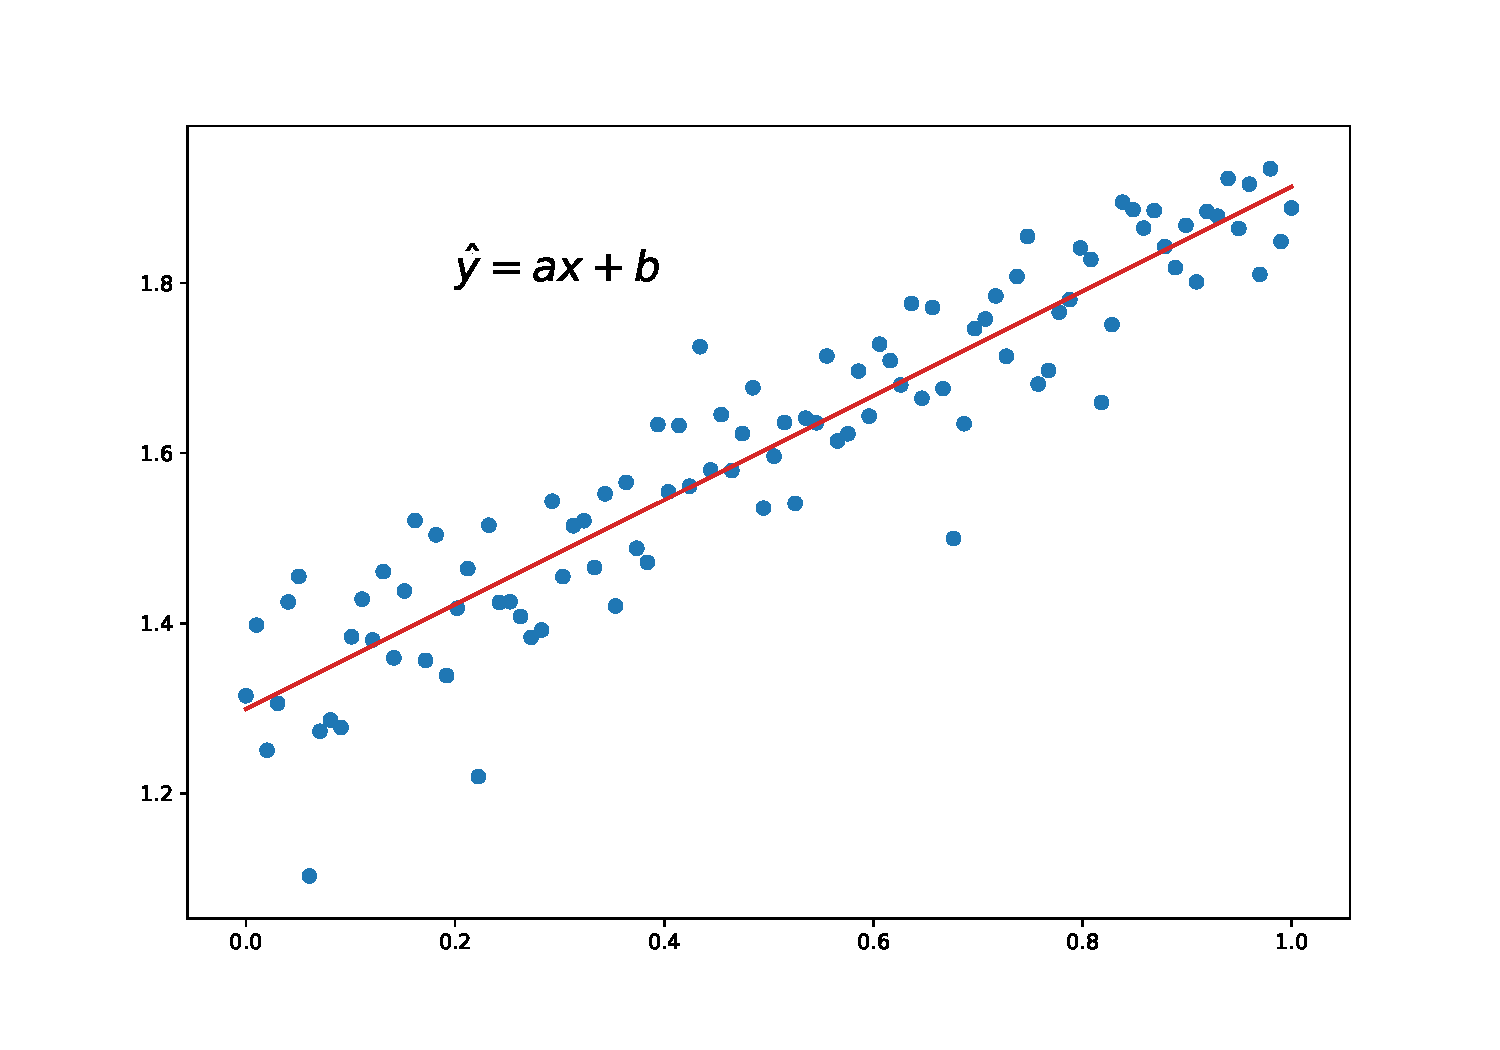
\includegraphics[width=0.7\textwidth]{lreg}
\caption{Regresión lineal simple. Consideramos una relación entre entre las variables dependientes $y$ e independientes $x$ dada por $\hat y = ax + b$}
\label{fig:simple_lreg}
\end{figure}

Sabiendo que $\{x_i\}_i$ y $\{y_i\}_i$ son los datos observados, minimizar $J(a, b)$ sería encontrar $a, b \in \Rnums$ que hace $J$ tan pequeña como sea posible.

\section{Un primer modelo: Regresión Lineal}
Como primer modelo de machine learning aprenderemos sobre la regresión lineal. Para motivar el uso de este modelo, supongamos queremos predecir las millas por galón (\textit{mpg}) de un coche dada una serie de variables las cuales, asumimos, afectan esta última. Para este problema estaremos trabajando con la serie de datos \texttt{mtcars} la cuál se encuentra en el cuadro \ref{table:mtcars} dentro de los apéndices.\\

En lenguaje de machine machine learning, decimos que este es un problema de regresión, es decir, el objetivo es encontrar una función $f:\Rnums^m \to \Rnums$. La variable \textit{mpg} es el \textit{target variable} y las variables de las cuales depende esta (en nuestro caso, número de cilindros, caballos de fuerza, etc.) son nuestros \textit{features}.\\

Para este modelo asumiremos que \textit{mpg} depende linealmente de las demás 10 variables más un coeficiente de corrección o \textit{bias term}\footnote{Este termino sería el equivalente a nuestro coeficiente $b$ para una regresión lineal simple.}. Es decir, nuestra predicción $\hat y$ está dada por:

\begin{equation}
	\hat y_i = \theta_0 + \theta_1x^{cyl}_i + \theta_2x^{disp}_i + \ldots + \theta_{10}x^{carbs}_i,
\end{equation}

donde $x_i^{cyl}$ representa $i$-ésima observación de la variable \textit{cyl}. De igual manera, $\hat y_i$ es la predicción echa por el modelo para la $i$-ésima observación. Mediremos el desempeño usando la función objetivo $J(\cdot)$\footnote{Recuerda que $J$ es la encargada de medir que tan \textit{mal} es nuestra predicción $\hat y_j$ con respecto al valor verdadero, $y_j$, para toda $j$},

\begin{equation}
J(\theta_0, \theta_1, \theta_2, \ldots, \theta_{10}) = \frac{1}{2}\sum_{n=1}^N(\theta_0 + \theta_1x^{cyl}_i + \theta_2x^{disp}_i + \ldots + \theta_{10}x^{carbs}_i - y_i)^2.
\end{equation}
 
 
 Para simplificar la notación agruparemos $\{\theta_i\}_{i=0}^{10}$ dentro del vector $\bm{\theta} \in \Rnums^{11}$, 
 
\begin{equation}
	\bm\theta = \begin{bmatrix}
	    \theta_0 \\
	    \theta_1 \\
	    \theta_2 \\
	    \vdots \\
	    \theta_{10}
	 \end{bmatrix}
\end{equation}

De igual manera, agruparemos la $j$-ésima observación dentro del vector $\bold{x}_j$,

\begin{equation}
\bold{x}_{j} = \begin{bmatrix}
            1 \\
            x^{cyl}_j \\
            x^{disp}_j \\
            \vdots \\
            x^{carbs}_j 
         \end{bmatrix}.
\end{equation}

Notemos que el primer elemento de $\bm{x}_j$ es una constante con valor $1$ ya que de esta manera podemos expresar $\hat y_j$ como

\begin{equation}
	\hat y_j = \bm{x}_j^T\bm\theta.
\end{equation}

Esta manera de expresar $\hat y_j$ nos lleva a reescribir nuestra función objetivo $J$ como una función en términos de un vector $\theta$, i.e.,

\begin{equation}
  J(\theta) = \frac{1}{2}\sum_{n=0}^N(\bm{x}_i^T\bm\theta - y)^2.
\end{equation}

Con ayuda del algebra lineal podemos simplificar $J(\bm\theta)$ a modo de trabajar con vectores y matrices. Consideremos cada observación $\{\bm{x}_n\}_{n=1}^N$ dentro de una matriz $\bm X\in\Rnums^{N\times m}$. Podemos considerar esta matriz resultante como la matriz de los datos presentados en el cuadro \ref{table:mtcars} con la adición de una columna $1$ para incluir el termino de corrección y sin considerar \textit{mpg}. De esta manera, $\bm X$ quedaría como sigue

\begin{align}
	 \bm{X} &= \begin{bmatrix}
	 	\bm{x}_1^T \\
	 	\bm{x}_2^T \\
	 	\vdots \\
	 	\bm{x}_N^T
	     \end{bmatrix}\\
	 &= \begin{bmatrix}
	        1 & x^{cyl}_1 & \ldots & x^{carbs}_1 \\
	        1 & x^{cyl}_2 & \ldots & x^{carbs}_2 \\
	        \vdots & \vdots & \ddots & \vdots\\
	        1 & x^{cyl}_N & \ldots & x^{carbs}_N \\
	     \end{bmatrix}
\end{align}

Para $N$ observaciones, nuestra estimación $\hat{\bm y} = \bm{X}\bm{\theta} \in \Rnums^{N}$.

Recordando que la norma $L_2$ de un vector $\bm{a}\in\Rnums^n$ se define

\begin{equation}
  ||\bm{a}||_2 = \sqrt{\bm{a}^T \bm{a}}
\end{equation}

Notamos que $J(\bm\theta)$ puede ser escrita como el cuadrado de la norma $L_2$ entre nuestras estimaciones y los valores observados, i.e., 
\begin{align}
	J(\bm\theta) &= ||\hat{\bm{y}} - \bm{y}||_2^2 \\
	          &=   ||\bm{X}\bm{\theta}^T - \bm{y}||_2^2
\end{align}

Lo que nos lleva a la representación final de la función objetivo $J(\bm\theta)$. Dada esta representación, el siguiente paso es encontrar el vector $\bm\theta^*$ que haga $J(\bm\theta)$ tan pequeño como sea posible. Para esto, será necesario hacer un análisis de la función objetivo.\\

Empecemos recordando qué encontrar $\bm\theta^*$ tal que $\nabla f(\bm\theta^*)= \bm{0}$ es encontrar un punto estacionario, i.e., $\bm\theta^*$ es un punto máximo, un punto mínimo o un punto de curvatura. Por las condiciones de segundo orden de convexidad, si demostramos que $J$ es positiva semidefinida, tendríamos que $\bm\theta^*$ es un mínimo global.\\

\begin{figure}
	\centering
	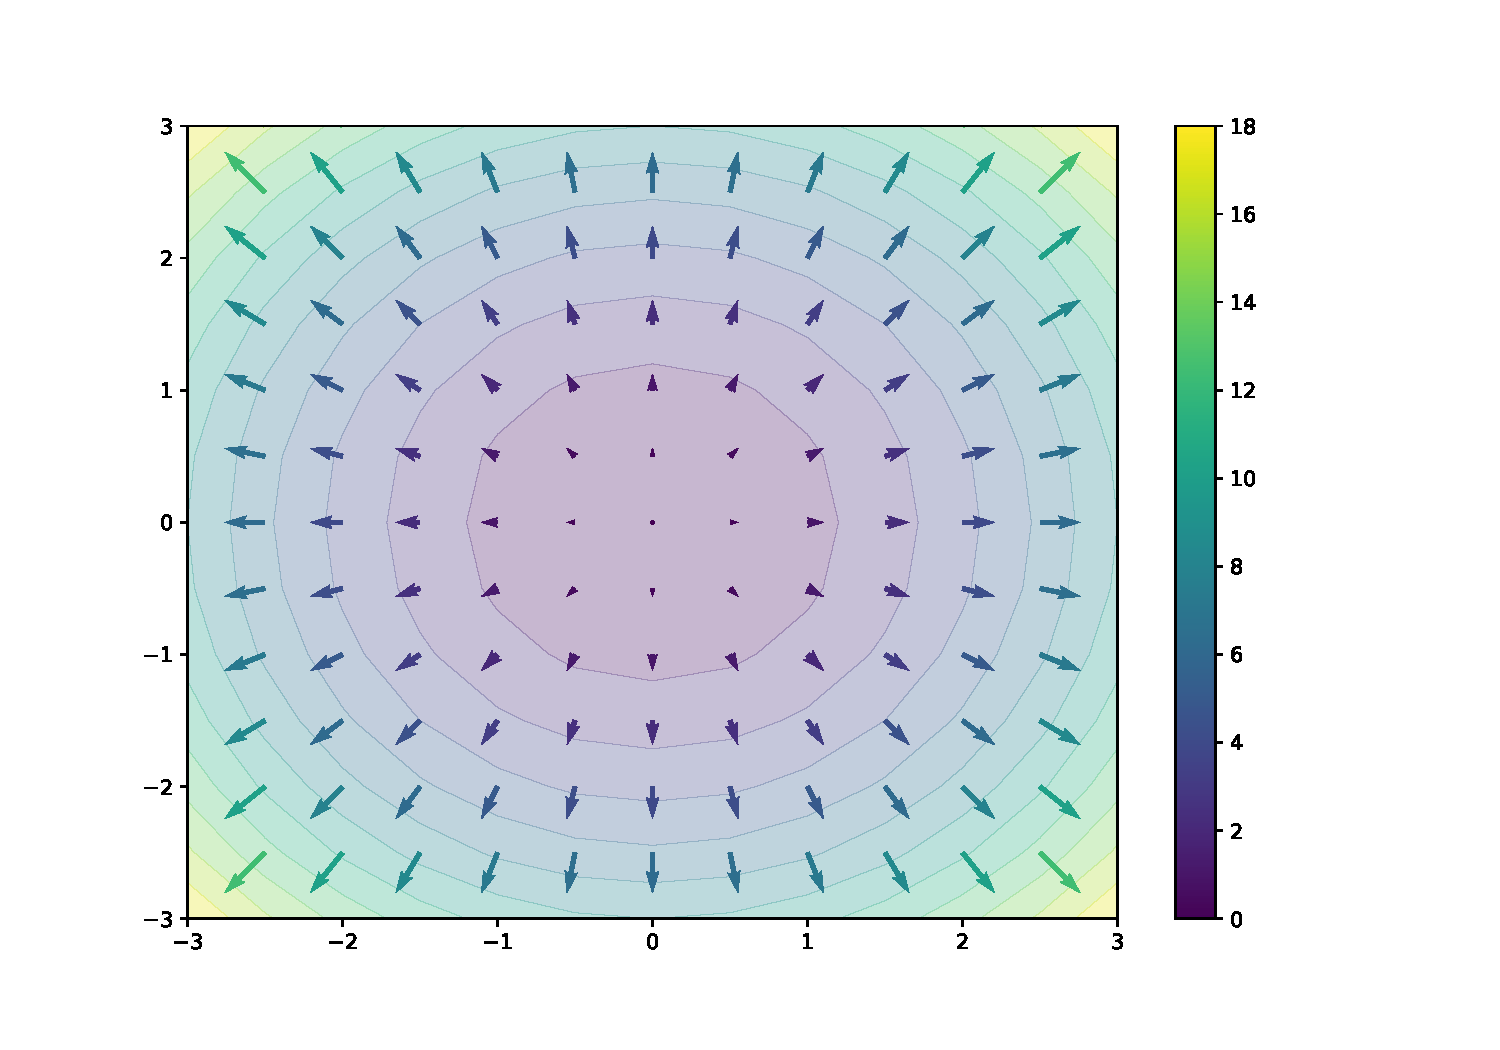
\includegraphics[width=0.8\textwidth]{grad}
	\caption{Mapa de gradientes para la función $f(x, y) = x^2 + y^2$. $\nabla f$ es un vector que indica que tan rápido la función crece (o decrece) para cada par $(x,y) \in\Rnums^2$. Encontrar donde $\nabla f(x^*, y^*) = \bm{0}$ es encontrar las coordenadas donde la función no crece ni decrece.}
\end{figure}

Empecemos por reescribir $J(\bm\theta)$ como sigue

 \begin{align}
   J(\bm\theta) &= \frac{1}{2}||\bm{X}\bm{\theta} - \bm{y}||_2^2\\
             &= \frac{1}{2}(\bm{X}\bm{\theta} - \bm{y})^T(\bm{X}\bm{\theta} - \bm{y})\\
             &= \frac{1}{2}\left(\bm{\theta}^T\bm{X}^T\bm{X}\bm{\theta} - 2\bm{\theta}^T\bm{x}^T\bm{y} + \bm{y}^T\bm{y}\right)\\
\end{align}

El gradiente de $J$ estaría dado por

\begin{align}
	\nabla J(\bm\theta) &= \nabla\frac{1}{2}\left(\bm{\theta}^T\bm{X}^T\bm{X}\bm{\theta} - 2\bm{\theta}^T\bm{x}^T\bm{y} + \bm{y}^T\bm{y}\right)\\
	&= \frac{1}{2}\left(2\bm{X}^T\bm{X}\bm{\theta} - 2 \bm{X}^T\bm{y}\right)\\
	&= \bm{X}^T\bm{X}\bm{\theta} - \bm{X}^T\bm{y}
\end{align}

Subsecuentemente tendríamos que el Hessiano es constante y está dado por
\begin{equation}
	\nabla^2 J(\bm\theta) = \bm{X}^T\bm{X}
\end{equation}

La cual es conocida como la matriz Gramiana y tiene la propiedad de ser posiva semidefinida. Esto anterior indica que existe por lo menos un mínimo global.  Asumiendo que las columnas de $\bm X$ son linealmente independientes, podemos resolver analíticamente $\nabla J(\bm\theta) = \bm 0$ que es fácil ver tiene como resultado

\begin{equation}\label{eq:normeq}
  \bm\theta^* = \left(\bm X^T\bm X\right)^{-1} \bm{X}^T\bm y
\end{equation}

Considerando la base de datos para nuestro problema y la ecuación \ref{eq:normeq}, observamos que el vector $\bm\theta^*$ resultante es

\begin{center}
\begin{tabular}{lr}
Parámetro & coeficiente\\
\midrule
\texttt{bias} & 12.303\\
 \texttt{cyl} & -0.111 \\
\texttt{disp} & 0.013 \\ 
  \texttt{hp} & -0.021 \\
\texttt{drat} & 0.787 \\
  \texttt{wt} & -3.715\\
\texttt{qsec} & 0.821\\
  \texttt{vs} & 0.318\\
  \texttt{am} & 2.520\\
\texttt{gear} & 0.655\\
\texttt{carb} & -0.199\\
\end{tabular}
\end{center}

Con $J(\bm\theta^*) \approx 147.49443$.\\

Dado $\bm\theta^*$, nos quedan dos cuestiones por resolver,
\begin{enumerate}
	\item ¿Qué tan bueno es el valor 147.49443?, ¿Podríamos mejorarlo considerando menos o más variables?;
	\item ¿Qué tanto el modelo refleja la realidad de los datos? Es decir, si tuviéramos datos sobre los cuáles no entrenamos el modelo, ¿sería el error encontrado muy cerca $147$?
\end{enumerate}

La primera cuestión hace referencia a la búsqueda del modelo óptimo; la segunda al problema de la \textbf{generalización}, un tema de gran importancia en el aprendizaje de máquina.

\section*{Ejercicios}
\begin{enumerate}
	\item Piensa en otra clase de tareas \textbf{T} y explícala.
	\item Considera tres problemas de \textit{unsupervised learning} y tres de \textit{supervised learning}. Anótalos y explica por qué caerían dentro de cada familia de problemas.
	\item Dada la función objetivo  $J(a, b) = \frac{1}{2}\sum_{i=1}^n(ax_i + b - y_i)^2$, ¿cuáles son los parámetros $a$, $b$ que minimizan la función? Resuelve el problema sin usar el gradiente.
	\item Demuestra que $\nabla_\theta(\theta^T Xy) = Xy$; $\theta\in\Rnums^m$, $X\in\Rnums^{m\times n}$ y $y\in\Rnums^n$. Recuerda que todo vector es considerado un vector columna.
	\item Convéncete que $\nabla_\theta(\theta^TXX^T\theta) = 2XX^T\theta$ considerando $X\in\Rnums^{2\times 2}$ y $\theta\in\Rnums^2$. ¿Cuál es el resultado de $\theta^TXX^T\theta$? Expresa tu resultado explícitamente (Hint: es un número real) ¿Cuál es resultado de calcular la parcial de $\theta^TXX^T\theta$ respecto a $\theta_0$ y $\theta_1$? ¿Cuál es el resultado de $2XX^T\theta$? (expresa tu resultado explícitamente)
\end{enumerate}

\newpage
\begin{appendices}
\begin{table}[h!]
\centering
\begin{tabular}{lrrrrrrrrrrr}
\toprule
{} &   mpg &  cyl &   disp &   hp &  drat &     wt &   qsec &  vs &  am &  gear &  carb \\
\midrule
Mazda RX4           &  21.0 &    6 &  160.0 &  110 &  3.90 &  2.620 &  16.46 &   0 &   1 &     4 &     4 \\
Mazda RX4 Wag       &  21.0 &    6 &  160.0 &  110 &  3.90 &  2.875 &  17.02 &   0 &   1 &     4 &     4 \\
Datsun 710          &  22.8 &    4 &  108.0 &   93 &  3.85 &  2.320 &  18.61 &   1 &   1 &     4 &     1 \\
Hornet 4 Drive      &  21.4 &    6 &  258.0 &  110 &  3.08 &  3.215 &  19.44 &   1 &   0 &     3 &     1 \\
Hornet Sportabout   &  18.7 &    8 &  360.0 &  175 &  3.15 &  3.440 &  17.02 &   0 &   0 &     3 &     2 \\
Valiant             &  18.1 &    6 &  225.0 &  105 &  2.76 &  3.460 &  20.22 &   1 &   0 &     3 &     1 \\
Duster 360          &  14.3 &    8 &  360.0 &  245 &  3.21 &  3.570 &  15.84 &   0 &   0 &     3 &     4 \\
Merc 240D           &  24.4 &    4 &  146.7 &   62 &  3.69 &  3.190 &  20.00 &   1 &   0 &     4 &     2 \\
Merc 230            &  22.8 &    4 &  140.8 &   95 &  3.92 &  3.150 &  22.90 &   1 &   0 &     4 &     2 \\
Merc 280            &  19.2 &    6 &  167.6 &  123 &  3.92 &  3.440 &  18.30 &   1 &   0 &     4 &     4 \\
Merc 280C           &  17.8 &    6 &  167.6 &  123 &  3.92 &  3.440 &  18.90 &   1 &   0 &     4 &     4 \\
Merc 450SE          &  16.4 &    8 &  275.8 &  180 &  3.07 &  4.070 &  17.40 &   0 &   0 &     3 &     3 \\
Merc 450SL          &  17.3 &    8 &  275.8 &  180 &  3.07 &  3.730 &  17.60 &   0 &   0 &     3 &     3 \\
Merc 450SLC         &  15.2 &    8 &  275.8 &  180 &  3.07 &  3.780 &  18.00 &   0 &   0 &     3 &     3 \\
Cadillac Fleetwood  &  10.4 &    8 &  472.0 &  205 &  2.93 &  5.250 &  17.98 &   0 &   0 &     3 &     4 \\
Lincoln Continental &  10.4 &    8 &  460.0 &  215 &  3.00 &  5.424 &  17.82 &   0 &   0 &     3 &     4 \\
Chrysler Imperial   &  14.7 &    8 &  440.0 &  230 &  3.23 &  5.345 &  17.42 &   0 &   0 &     3 &     4 \\
Fiat 128            &  32.4 &    4 &   78.7 &   66 &  4.08 &  2.200 &  19.47 &   1 &   1 &     4 &     1 \\
Honda Civic         &  30.4 &    4 &   75.7 &   52 &  4.93 &  1.615 &  18.52 &   1 &   1 &     4 &     2 \\
Toyota Corolla      &  33.9 &    4 &   71.1 &   65 &  4.22 &  1.835 &  19.90 &   1 &   1 &     4 &     1 \\
Toyota Corona       &  21.5 &    4 &  120.1 &   97 &  3.70 &  2.465 &  20.01 &   1 &   0 &     3 &     1 \\
Dodge Challenger    &  15.5 &    8 &  318.0 &  150 &  2.76 &  3.520 &  16.87 &   0 &   0 &     3 &     2 \\
AMC Javelin         &  15.2 &    8 &  304.0 &  150 &  3.15 &  3.435 &  17.30 &   0 &   0 &     3 &     2 \\
Camaro Z28          &  13.3 &    8 &  350.0 &  245 &  3.73 &  3.840 &  15.41 &   0 &   0 &     3 &     4 \\
Pontiac Firebird    &  19.2 &    8 &  400.0 &  175 &  3.08 &  3.845 &  17.05 &   0 &   0 &     3 &     2 \\
Fiat X1-9           &  27.3 &    4 &   79.0 &   66 &  4.08 &  1.935 &  18.90 &   1 &   1 &     4 &     1 \\
Porsche 914-2       &  26.0 &    4 &  120.3 &   91 &  4.43 &  2.140 &  16.70 &   0 &   1 &     5 &     2 \\
Lotus Europa        &  30.4 &    4 &   95.1 &  113 &  3.77 &  1.513 &  16.90 &   1 &   1 &     5 &     2 \\
Ford Pantera L      &  15.8 &    8 &  351.0 &  264 &  4.22 &  3.170 &  14.50 &   0 &   1 &     5 &     4 \\
Ferrari Dino        &  19.7 &    6 &  145.0 &  175 &  3.62 &  2.770 &  15.50 &   0 &   1 &     5 &     6 \\
Maserati Bora       &  15.0 &    8 &  301.0 &  335 &  3.54 &  3.570 &  14.60 &   0 &   1 &     5 &     8 \\
Volvo 142E          &  21.4 &    4 &  121.0 &  109 &  4.11 &  2.780 &  18.60 &   1 &   1 &     4 &     2 \\
\bottomrule
\end{tabular}
\caption{\texttt{mtcars} dataset}
\label{table:mtcars}
\end{table}
\end{appendices}

\newpage
\nocite{*}
\bibliography{ref}
\end{document}
